\begin{figure}[H]
  \centering
  \resizebox{\textwidth}{!}{
  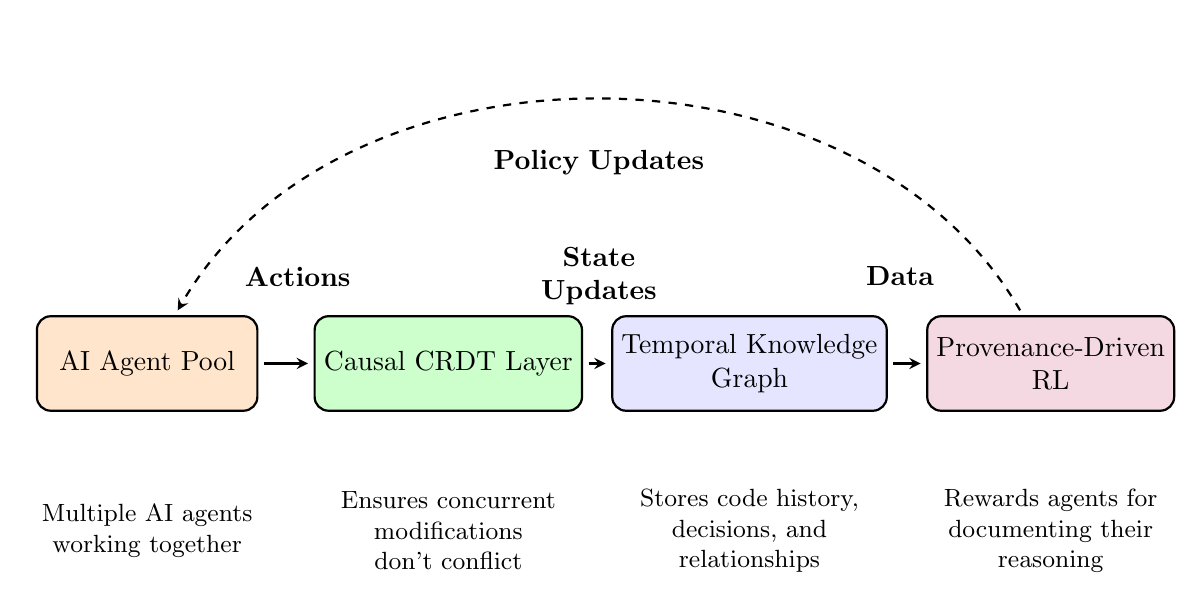
\begin{tikzpicture}[
    scale=0.85,
    box/.style={draw, minimum width=2.8cm, minimum height=1.2cm, align=center, rounded corners=5pt, thick},
    agent/.style={box, fill=orange!20},
    tkg/.style={box, fill=blue!10},
    crdt/.style={box, fill=green!20},
    rl/.style={box, fill=purple!15},
    arrow/.style={->, >=stealth, thick, shorten >=2pt, shorten <=2pt},
    dashedarrow/.style={->, >=stealth, thick, dashed, shorten >=2pt, shorten <=2pt}
  ]

  % Main components in a simple horizontal flow with increased spacing
  \node[agent] (agent) at (0,0) {AI Agent Pool};
  \node[crdt] (crdt) at (4.5,0) {Causal CRDT Layer};
  \node[tkg] (tkg) at (9,0) {Temporal Knowledge\\Graph};
  \node[rl] (rl) at (13.5,0) {Provenance-Driven\\RL};

  % Draw arrows without labels first
  \draw[arrow] (agent) -- (crdt);
  \draw[arrow] (crdt) -- (tkg);
  \draw[arrow] (tkg) -- (rl);

  % Add labels as separate nodes with improved spacing
  % Place 'Actions', 'State Updates', 'Data' above their respective arrows with more horizontal space
  
  % 'Actions' above agent->crdt
  \node[text width=2cm, align=center] at (2.25,1.3) {\textbf{Actions}};
  % 'State Updates' above crdt->tkg
  \node[text width=2.2cm, align=center] at (6.75,1.3) {\textbf{State Updates}};
  % 'Data' above tkg->rl
  \node[text width=2cm, align=center] at (11.25,1.3) {\textbf{Data}};

  % Feedback loop label: 'Policy Updates' centered above the dashed arrow, with extra vertical space for separation
  \node[text width=3cm, align=center] at (6.75,3.0) {\textbf{Policy Updates}};

  % Feedback loop with a higher arc to avoid overlapping 'Actions'
  \draw[dashedarrow] (rl) to[bend right=60] (agent);

  % Add a simple explanation of each component below with significantly increased vertical spacing
  \node[align=center, text width=2.8cm, font=\small] at (0,-2.5) {Multiple AI agents\\working together};
  \node[align=center, text width=2.8cm, font=\small] at (4.5,-2.5) {Ensures concurrent\\modifications\\don't conflict};
  \node[align=center, text width=2.8cm, font=\small] at (9,-2.5) {Stores code history,\\decisions, and\\relationships};
  \node[align=center, text width=2.8cm, font=\small] at (13.5,-2.5) {Rewards agents for\\documenting their\\reasoning};

  \end{tikzpicture}
  }
  \caption{Arc Architecture: A simplified view of how Arc's components work together. AI agents make changes through the Causal CRDT layer, which safely updates the Temporal Knowledge Graph. The Provenance-Driven RL component learns from this data and improves agent policies, creating a continuous improvement cycle.}
  \label{fig:arc_architecture}
\end{figure}
